
\documentclass[12pt,a4paper]{article}

\usepackage{color}
\usepackage{amsxtra}  
\usepackage{amsthm}
\usepackage{amssymb}
\usepackage{amsfonts}
\usepackage{graphicx}  
\usepackage{rotating}


\begin{document}

\title{Report: Summary of Simulation and Unsolved Problems}
\author{Wenwen Huang}
\date{\today}

\maketitle

In this report, I will summarize the recent results from simulations and the
problem we facing in theory. The simulation results refer both 3D Brownian
Dynamic simulation and 1D single-file diffusion simulation. For the theory, I
thought it was almost solved but it turns out not that easy. I would like to
state it here and we can discuss how to proceed next.

So firstly, I will briefly discuss the model we are using and the problem we
want to solve, and then I will summarize the simulation results, both 3D and
1D, last but not least, the progress on theory and unsolved problem is discussed
in detail.

\section{Relaxation of Chromosome Modeled as Pinned Polymer Loop}

As we know that chromosome in fission yeast during meiosis can be modeled by
pinned polymer loop. Previously, we solved the equilibrium statistics based on
this model. The result shows that the pulling behavior can significantly
decrease the distance of corresponding sites of homologous, providing the
physical condition for biological interactions. 

However, in real fission yeast, chromosomes are not pulling with constant
velocity in one direction. Instead, nucleus containing chromosomes is
oscillating, gives out a non-equilibrium process. So what we want to know now is
the non-equilibrium relaxation of chromosome, which is modeled by pinned polymer
loop. More precisely, given an arbitrary polymer configuration, we want to know
how it evolves to equilibrium, which we already know for different $\tilde{T}$.

\section{Simulation Results}
In this section, I will summarize the simulation results we have now. Of
course, further simulation can be done easily if needed. To demonstrate the
results, I will take three typical value of effective temperature, $\tilde{T} =
1, 10, \inf$, representing strong external force case, moderate external force
case and totally without external force case, respectively. And the number of
beads is $N = 100$ unless state otherwise. 

\subsection{3D Brownian Dynamic Simulation}
For 3D simulation, the setup is normal as usual. Predictor-Corrector algorithm
is adopted and pseudo-potential is included in all simulations. Moreover,
the movement of pinned bead is subtracted as offset. So now the polymer loop is
ideally pinned. 

In order not to mess things up, here I only discuss the relaxation of
$\left<z\right>$ component of bead position. Although we already have results
strongly hint the rich underlying physics of variance relaxation, correlation
between different directions, etc. We shall come to these topics later. By now
we just watch the parameter measures the distance to equilibrium defined as
following
\begin{equation}
    d_z = |\left<z\right>_t - \left<z\right>_{eq}|
\end{equation}

\subsubsection{Strong External Force Field ($\tilde{T} = 1$)}
For the case of strong external force field, we can evidently distinguish two
dynamic regimes (the second one of previous three regimes vanished because of
subtraction of pinned bead movement). 

The first one is linear. The underlying physical picture is following:
initially, the configuration is random, the beads feel the external force field
and moving along the force direction. As a result, we would expect the same
constant moving velocity for every bead, which is proved by the simulation data
in Fig.\ref{fig:bdt1}

The second regime is a exponential decay of the distance parameter. This is a
common relaxation process in many non-equilibrium processes. The point here 
is that although the distance to equilibrium is different for beads near pinned
one or far from pinned one, it looks like they have the same exponent
characterizing this regime, see in Fig.\ref{fig:bdt1}.

\begin{figure}[htpb]
    \centering
    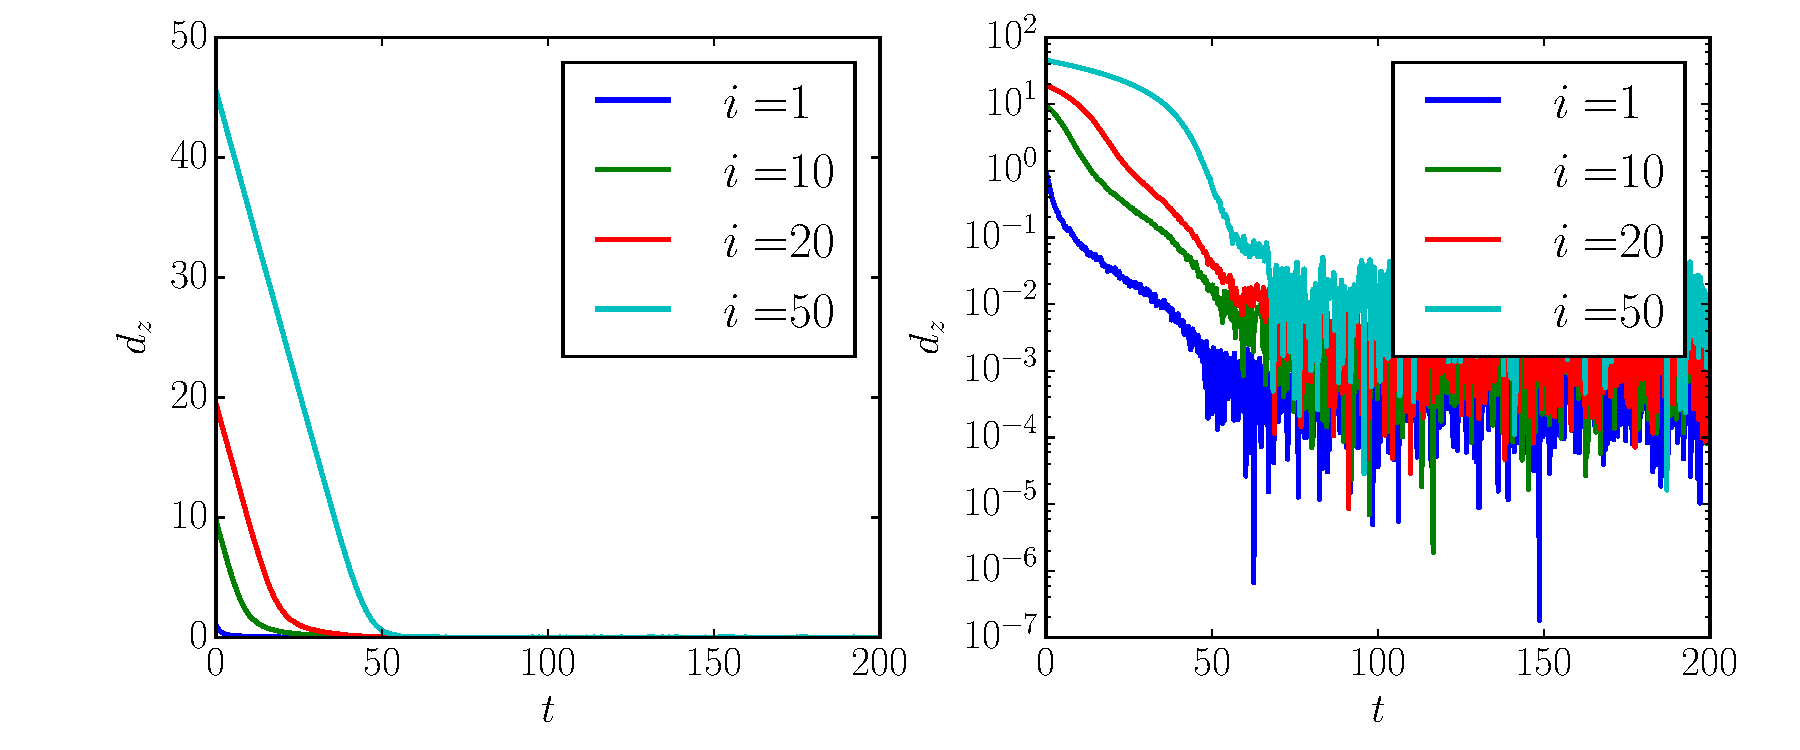
\includegraphics[width=1.0\linewidth]{fig4report/bd_N100_T1_un.pdf}
    \caption{ Relaxation process for $\tilde{T}=1$, left panel is linear plot,
        right panel is log-linear plot. $i$ is the index of bead, number of
        beads $N=100$. From the left panel we can see the initial slope of all
        beads are the same, which means that all beads moving in the same
        constant velocity.}
    \label{fig:bdt1}
\end{figure}

\subsubsection{Moderate External Force Field ($\tilde{T} = 10$)}
The same two regime relaxation is also seen for the case of moderate external
force field. The difference comparing to $\tilde{T} = 1$ is that the linear
regime becomes less distinguished, and the normalized curves of $d_z$ for
different bead are much more closer to each other, see Fig. \ref{fig:bdt10}.
However, we still notice that the bead far from pinned one (such as $i=50$)
relax slower than other ones. And this is due to a longer linear regime as the
initial configuration is random.
\begin{figure}[htpb]
    \centering
    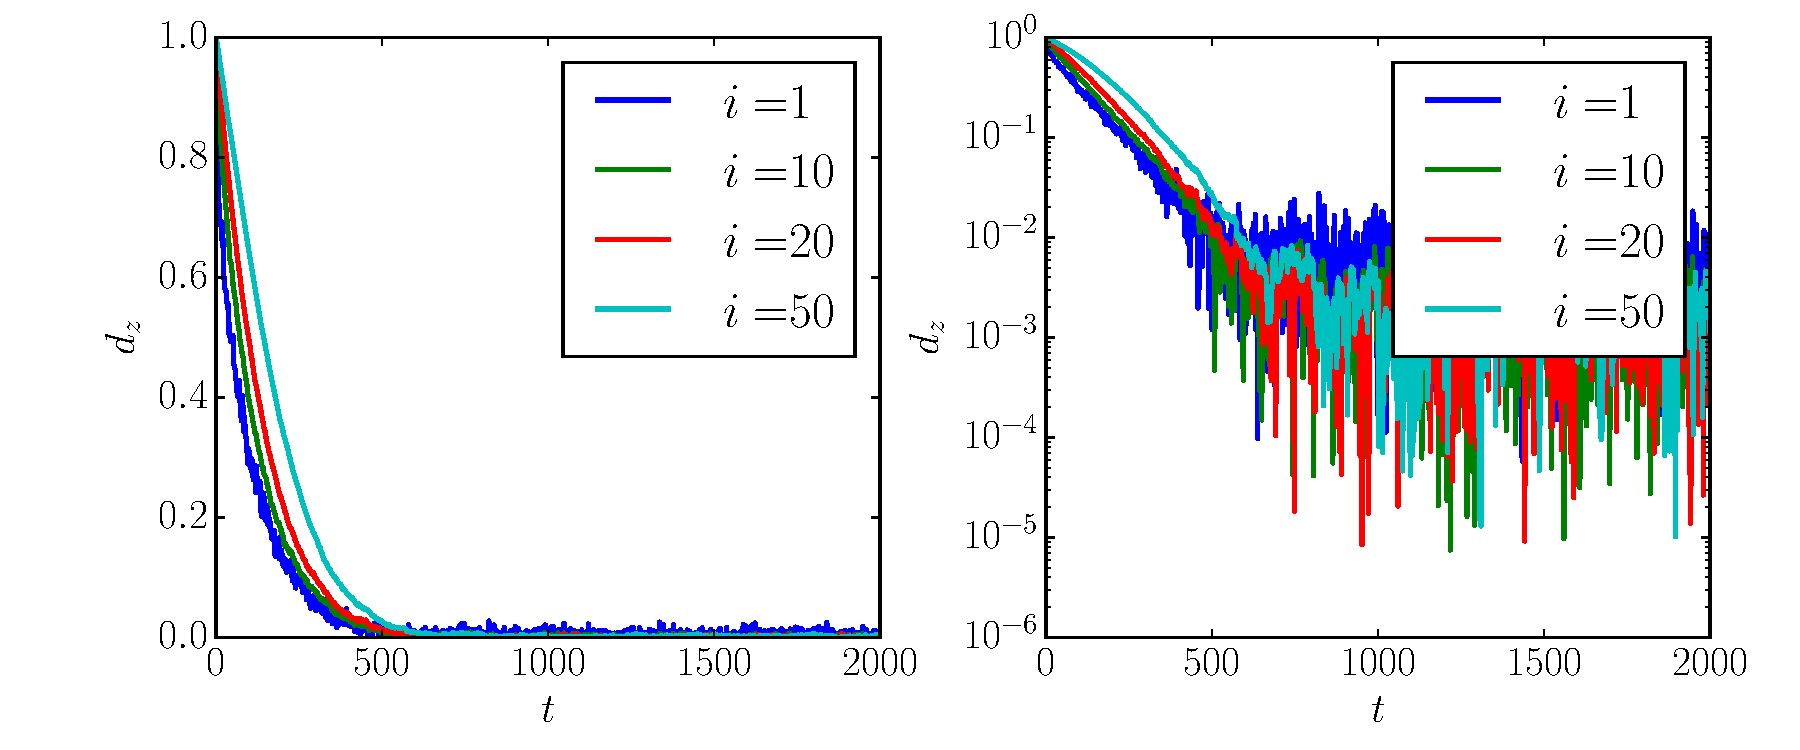
\includegraphics[width=1.0\linewidth]{fig4report/bd_N100_T10.pdf}
    \caption{Relaxation process for $\tilde{T}=10$, $d_z$ is normalized. The
        universal exponent for different beads is more obviously see for this
        case. Notice bead $i=50$ still relax slowest in this case.}
    \label{fig:bdt10}
\end{figure}

\subsubsection{No External Force Field ($\tilde{T}=\inf$)}
For the case totally without external force field, we can not start from the
random initial configuration. Because this is already the equilibrated state.
Instead, the fully stretched initial configuration along the force field is used
in the simulation. Interesting thing here is that, unlike previous cases of
$\tilde{T}=1$ or $\tilde{T}=10$, beads far from the pinned one relax faster than
other ones, see in Fig.\ref{fig:bdtinf}.

\begin{figure}[htpb]
    \centering
    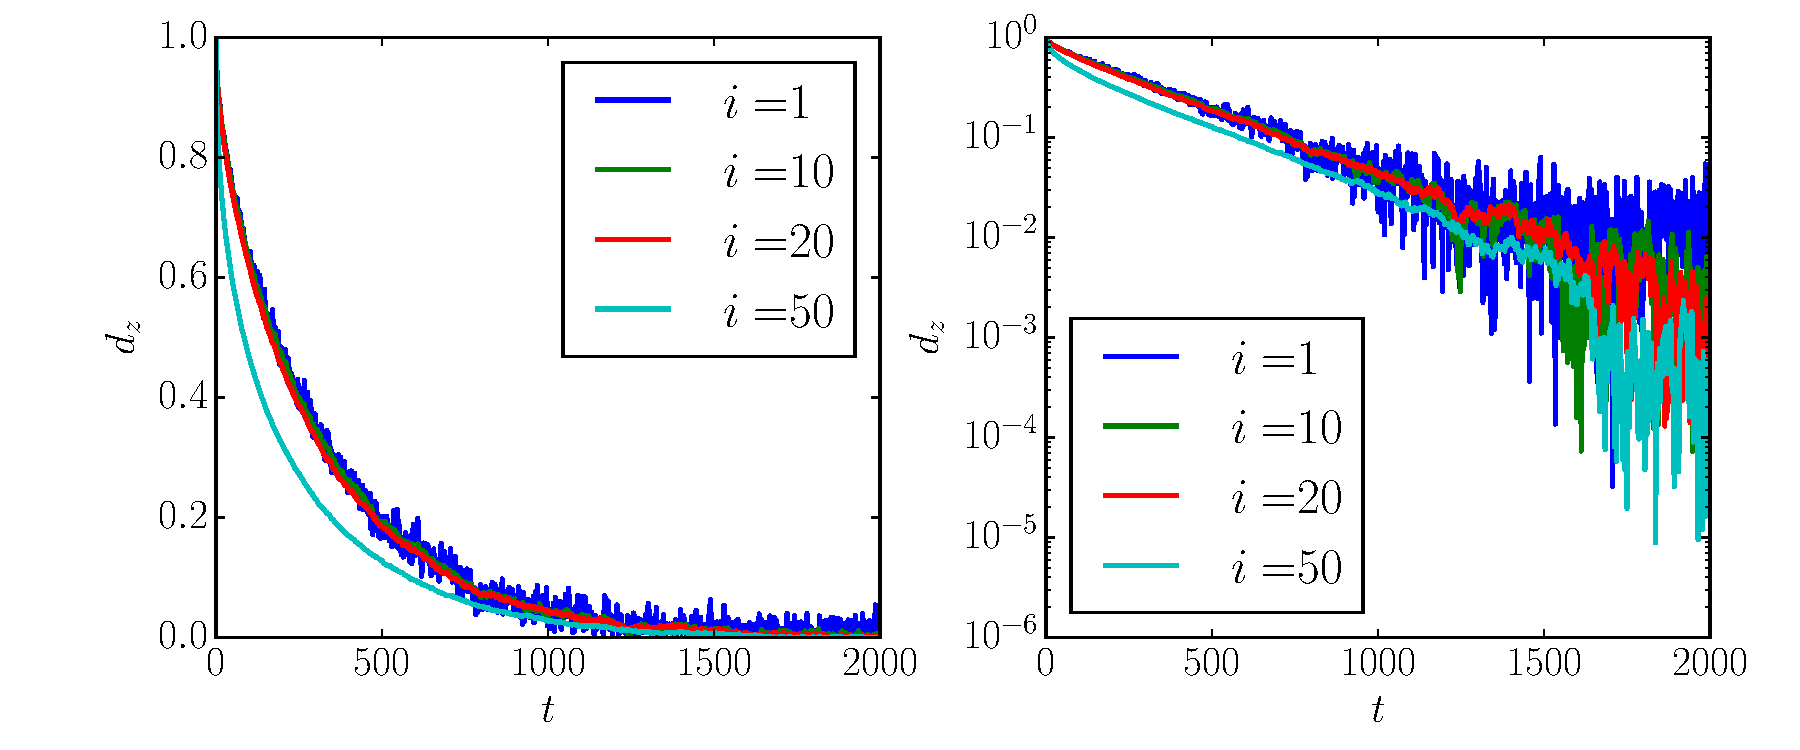
\includegraphics[width=1.0\linewidth]{fig4report/bd_N100_Tinf.pdf}
    \caption{Relaxation process for $\tilde{T}=\inf$, $d_z$ is normalized.
        Notice bead $i=50$ relax faster than other beads in this case.} 
    \label{fig:bdtinf}
\end{figure}
My explanation for this phenomenon is as following: when we start from a
stretched configuration, the freedom of movement for beads near the pinned one
is constrained. For example, it would be harder for the tail part of polymer to
rotate according to the axis go across bead $i=10$ than according to the axis go
across $i=49$. On the other hand, the freedom movement for beads far from the
pinned one is less constrained, so the initial relaxation of these beads goes
faster. We can also get hints from the 1D simulation result shown in section
\ref{sec:1dtinf}.

\subsection{1D Kinetic Monte Carlo Simulation}
As we know, the configuration of 1D polymer loop can exactly map to
configuration of $N/2$ particle sitting on $N$ lattice sites, with constraint
that one site can be occupied by no more than one particle. So our working idea
is the dynamics of polymer configuration can be mapped to the diffusion of such
single file system. To check the idea, we do 1D Kinetic Monte Carlo simulation
on a particle hopping model, and map it back to the polymer configuration to
measure the relaxation, and then compare it with the 3D polymer relaxation
behavior, to see whether they are similar or not.  

We again check the simulation results of three typical value of $\tilde{T}$ in
1D. The setup of the simulation is a typical particle hopping model (ASEP). A
randomly selected particle would hop to left or right if the site is not
occupied. The hopping rate $\mu$ with subscript indicates hopping direction is
related to the parameter $\tilde{T}$, and can be written as:
\begin{eqnarray}
    \mu_{right} & = &
    c\frac{\exp{(-\frac{1}{\tilde{T}}})}{1+\exp{(-\frac{1}{\tilde{T}}})} \\
    \mu_{left} & = & c\frac{1}{1+\exp{(-\frac{1}{\tilde{T}}})}
\end{eqnarray}
where $c$ is a constant related to the level of noise which is set be $1$ in
this simulation.

\subsubsection{Strong External Force Field ($\tilde{T}=1$)}
We plot the same figure as in 3D simulation. In the case of strong external
force field, we see very similar relaxation process as 3D polymer system.
Specifically, a linear regime that all beads moving in constant speed is
followed by a exponential regime where the exponent is irrelevant of bead index,
see in Fig. \ref{fig:asept1}.
\begin{figure}[htpb]
    \centering
    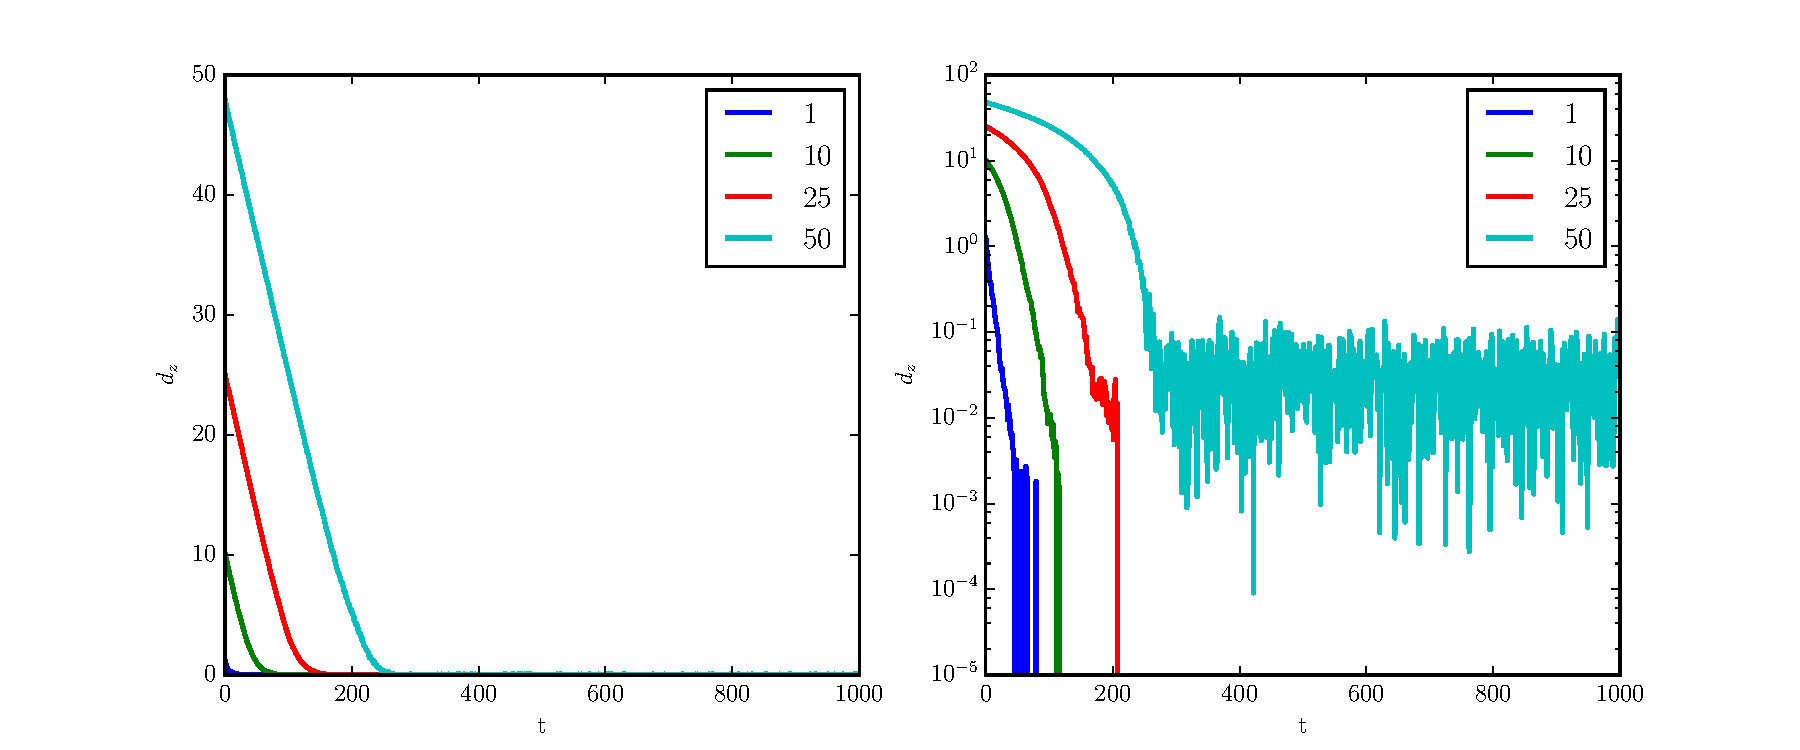
\includegraphics[width=1.0\linewidth]{fig4report/asep_N100_T1_un.pdf}
    \caption{Relaxation process for $\tilde{T}=1$, $d_z$ is unnormalized.} 
    \label{fig:asept1}
\end{figure}

\subsubsection{Moderate External Force Field ($\tilde{T} = 10$)}
Again, a very similar relaxation process to 3D is observed in case moderate
external force field, see in Fig. \ref{fig:asept10}.
\begin{figure}[htpb]
    \centering
    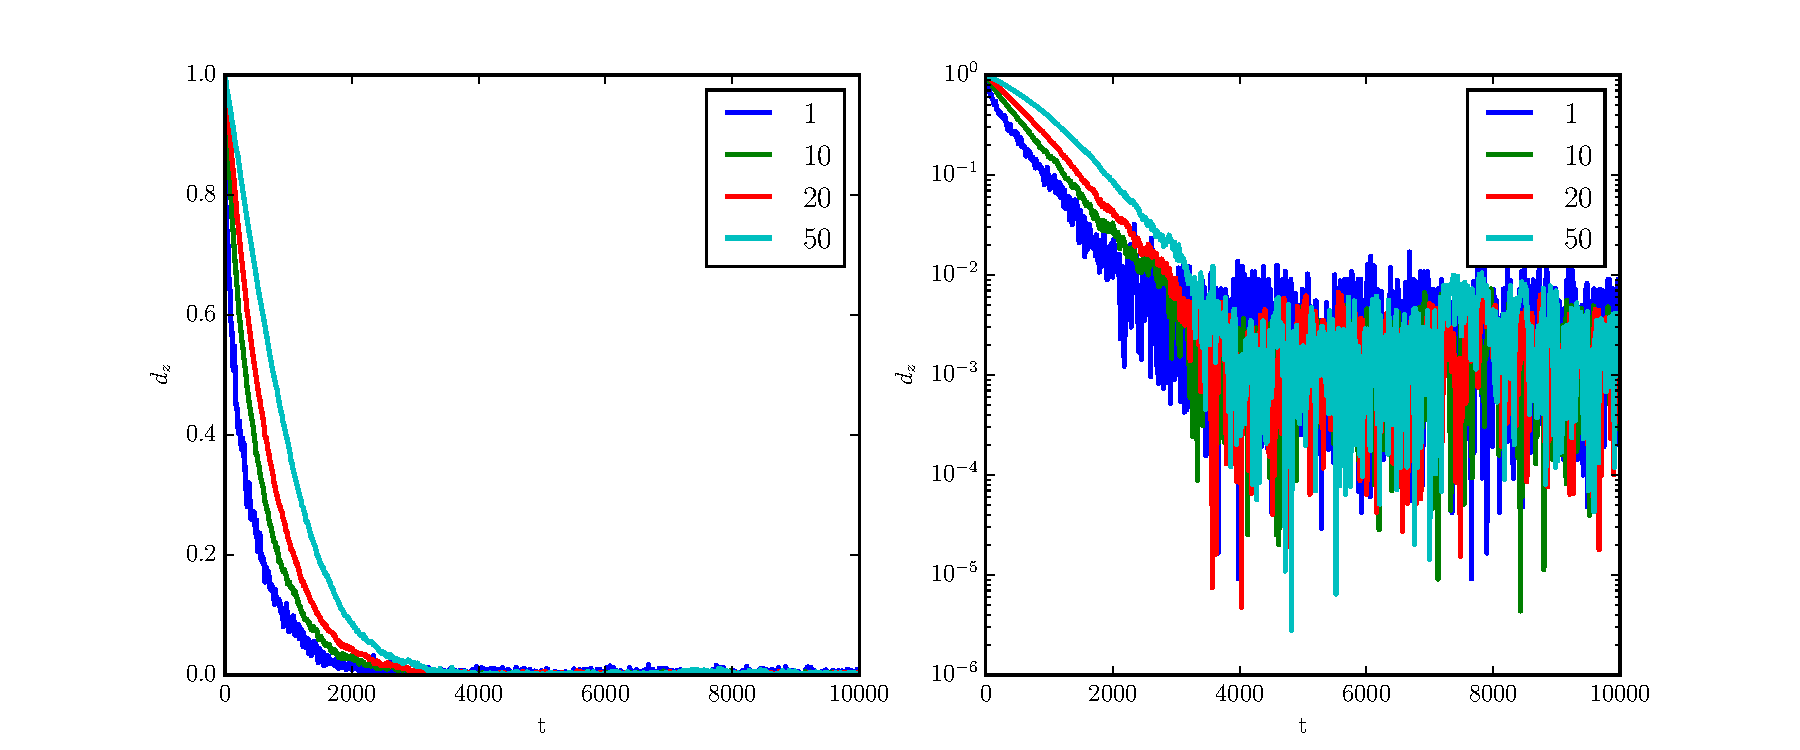
\includegraphics[width=1.0\linewidth]{fig4report/asep_N100_T10.pdf}
    \caption{Relaxation process for $\tilde{T}=10$, $d_z$ is normalized.
        Notice bead $i=50$ relax faster than other beads in this case.} 
    \label{fig:asept10}
\end{figure}

\subsubsection{No External Force Field ($\tilde{T}=\inf$)}
\label{sec:1dtinf}
For the case without external force field, we already see in 3D that the bead
far from pinned bead would relax faster. This is again verified in the 1D
simulation, see in Fig. \ref{fig:aseptinf}. In this case, we can see deeper why
the tail part of beads relax faster. Think about that we start with fully stretched
configuration, in particle diffusion picture, this corresponds to all the
particles are sitting on the left half sites of the 1D lattice. In this case,
because of the exclusive constraint, only the rightmost particle can move, which
means that only the bead at the tail part relax. We can verify this to zoom in
the beginning part of the unnormalized $d_z$ case, see in Fig.
\ref{fig:aseptinfun}. A plateau is seen for those beads not at the tail part,
which indicates these beads do not move at beginning.
\begin{figure}[htpb]
    \centering
    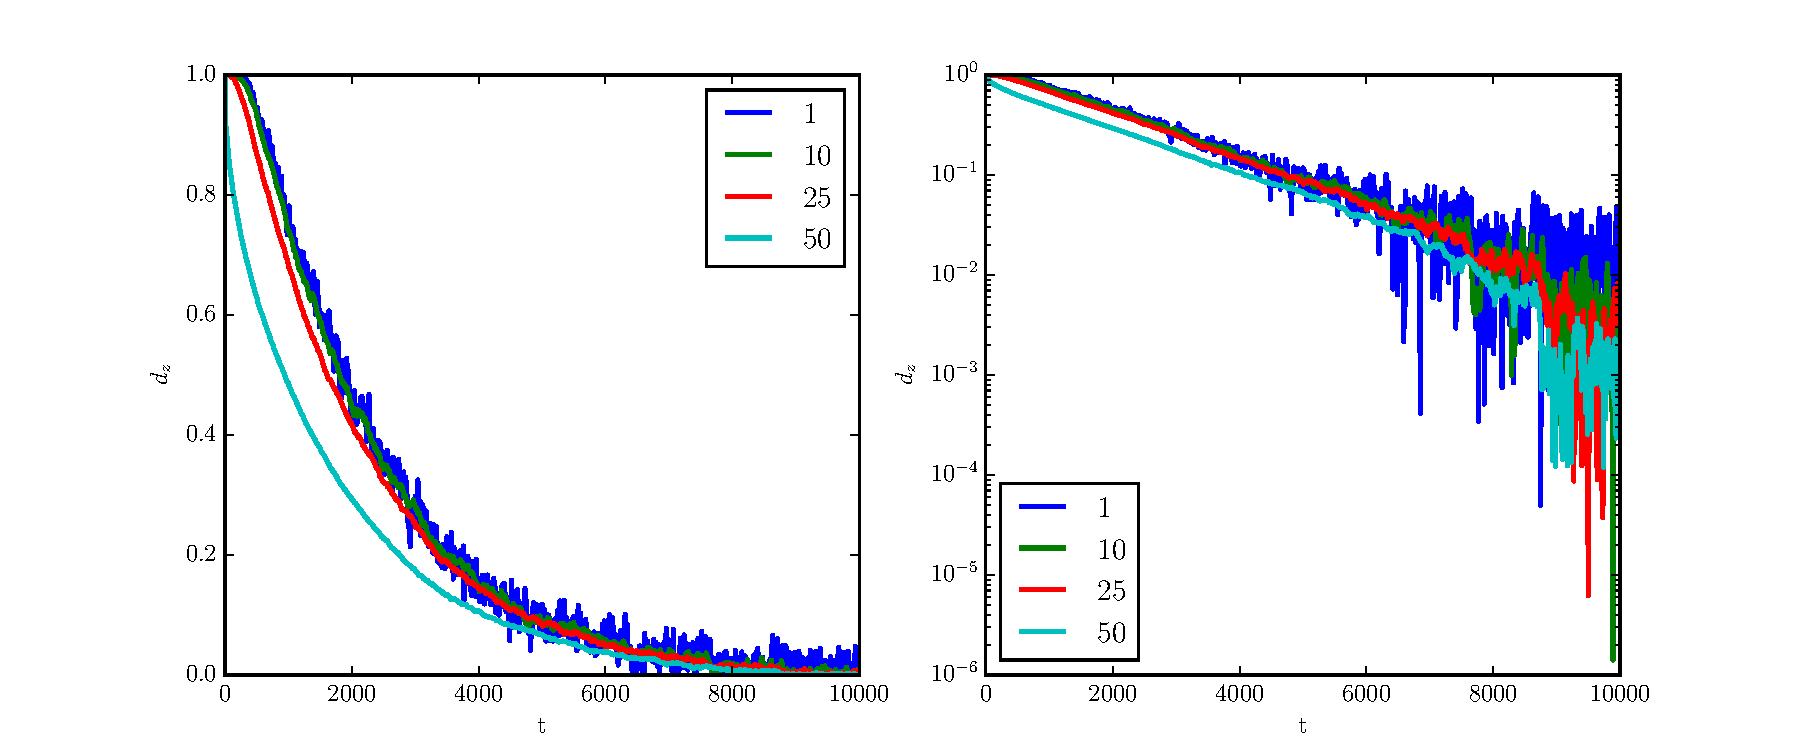
\includegraphics[width=1.0\linewidth]{fig4report/asep_N100_Tinf.pdf}
    \caption{Relaxation process for $\tilde{T}=\inf$, $d_z$ is normalized.
        Notice bead $i=50$ relax faster than other beads in this case.} 
    \label{fig:aseptinf}
\end{figure}

\begin{figure}[htpb]
    \centering
    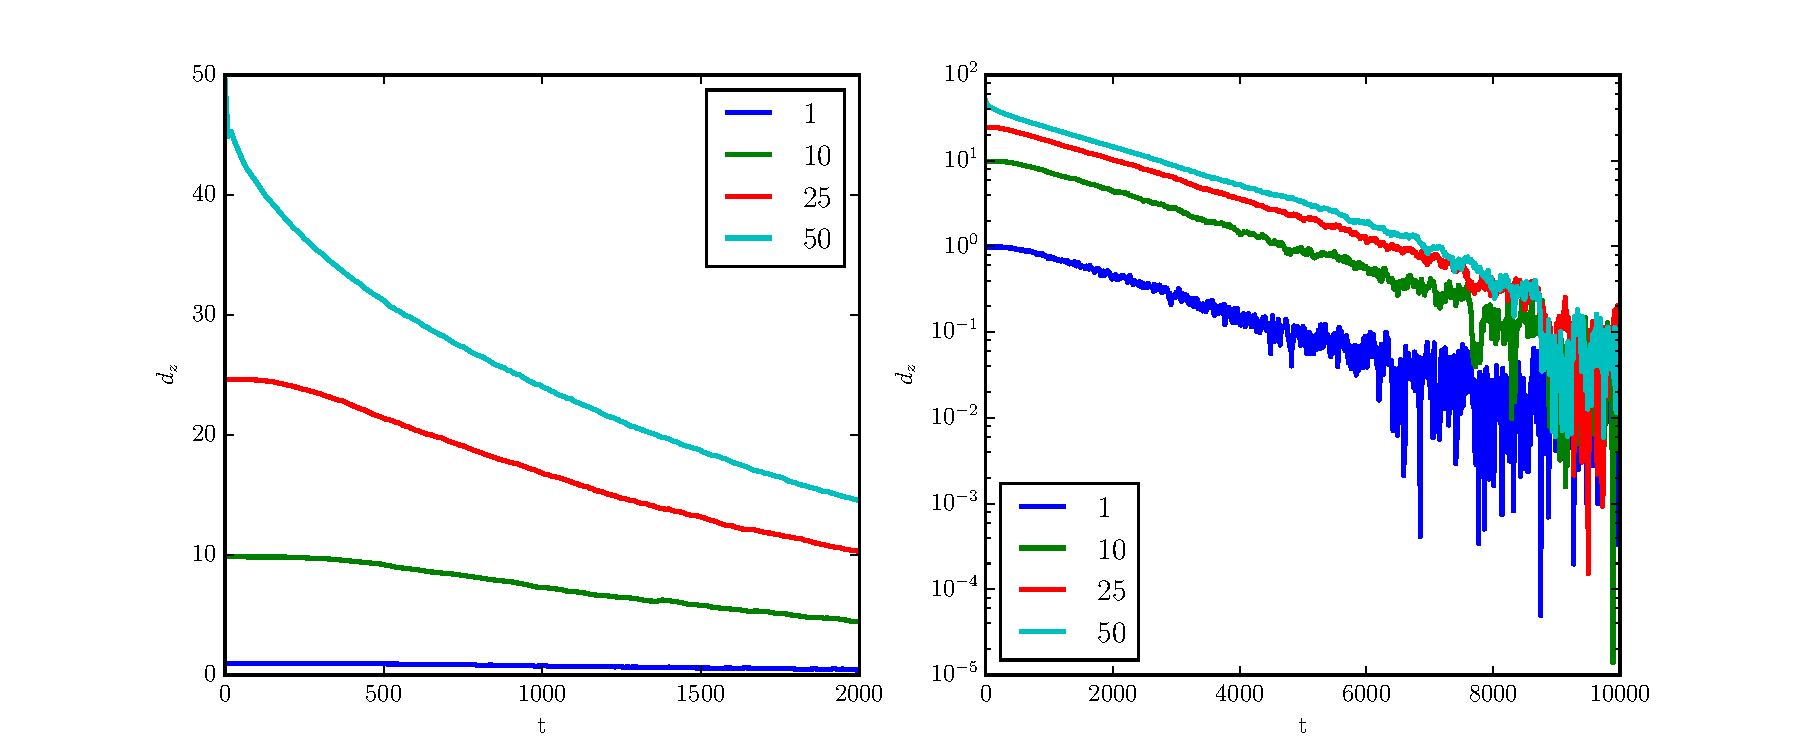
\includegraphics[width=1.0\linewidth]{fig4report/asep_N100_Tinf_un.pdf}
    \caption{Relaxation process for $\tilde{T}=\inf$, $d_z$ is unnormalized.
        Notice a plateau at the beginning of curves is seen in the left panel.} 
    \label{fig:aseptinfun}
\end{figure}

\subsection{Relaxation Time for Different $\tilde{T}$}
Ultimately, we want to know how is the relaxation time of polymer system changes
with the parameter $\tilde{T}$. The simulation results for this can be done both
in 3D and 1D by fitting the exponent of the second relaxation regime. By now,
the accuracy of the fitting is maybe not perfect but still valid to estimate the
tendency for relaxation time $\tau$ varies with $\tilde{T}$. Result of 3D is
shown in Fig. \ref{fig:bdtemptau} and 1D in Fig. \ref{fig:aseptemptau}.

As we can see from the two figures, they are actually very similar to each other
except a pre-factor. Notice here, I only plot the fitting results for $\tilde{T}
\leqslant 100$, for $\tilde{T} > 100$ something different happen, relaxation
time decreases. I still have to check this is because of fitting error or there
are some deep exciting physics inside.
\begin{figure}[htpb]
    \centering
    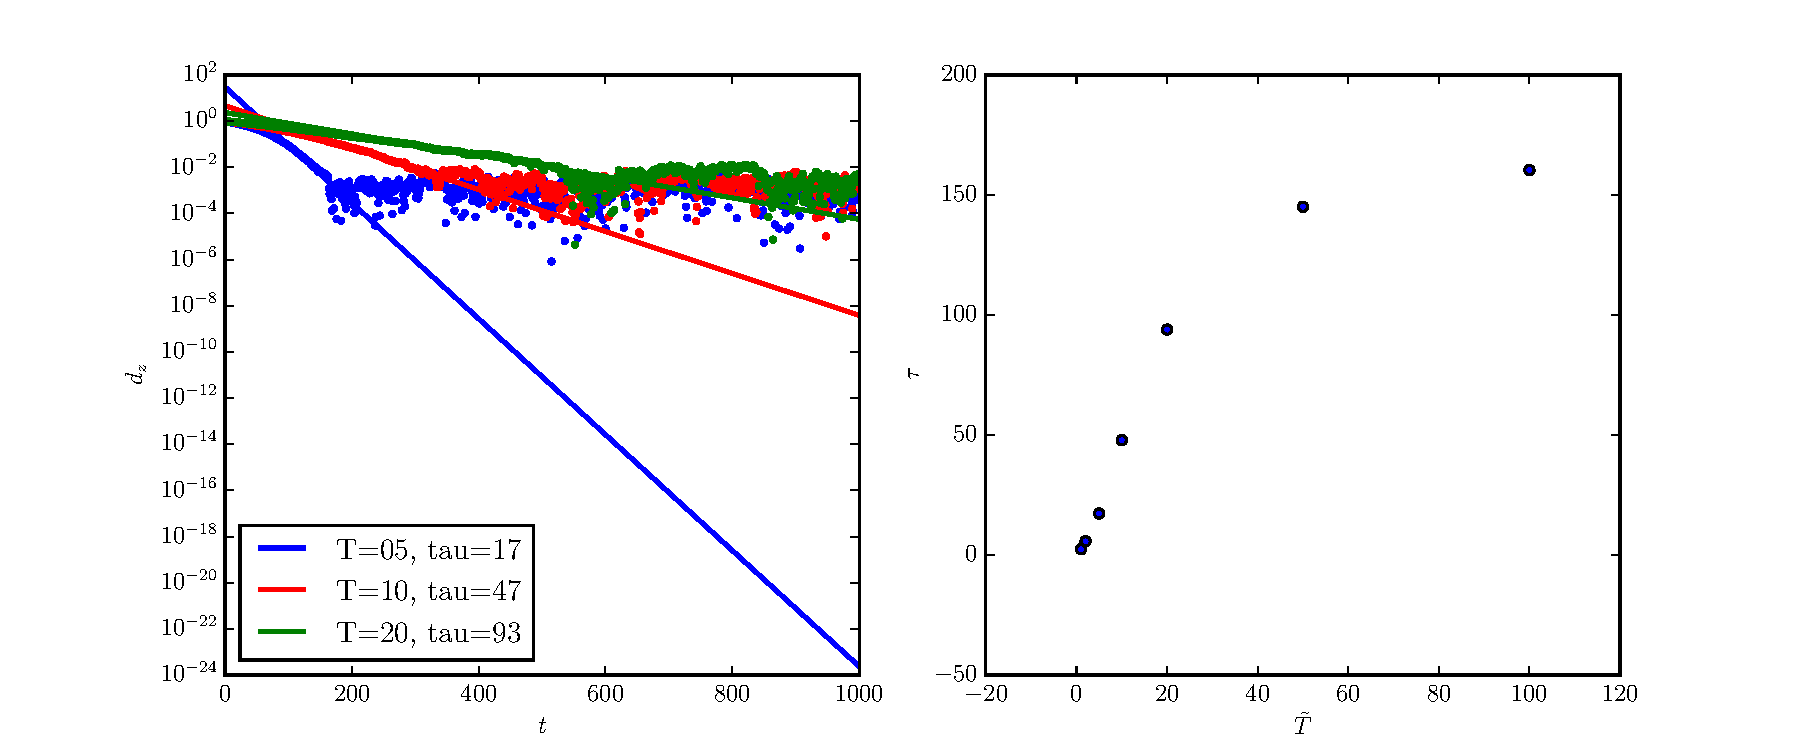
\includegraphics[width=1.0\linewidth]{fig4report/bdTempTau.pdf}
    \caption{Relaxation time varies with $\tilde{T}$ in 3D simulation. Left
        panel illustrate the fitting in several case, right panel shows the
        result for different $\tilde{T}$.} 
    \label{fig:bdtemptau}
\end{figure}

\begin{figure}[htpb]
    \centering
    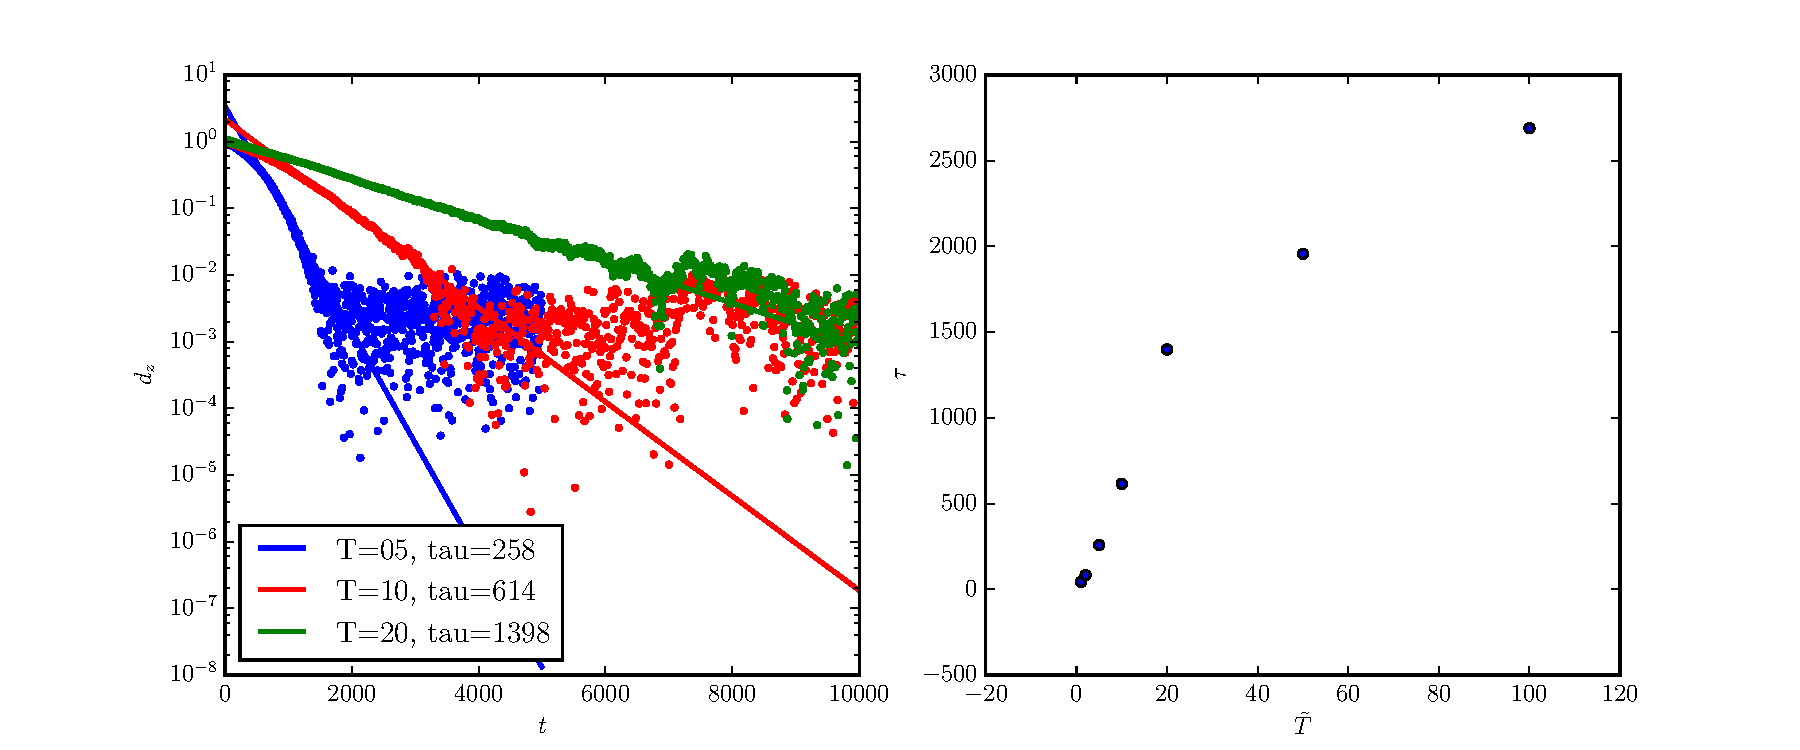
\includegraphics[width=1.0\linewidth]{fig4report/asepTempTau.pdf}
    \caption{Relaxation time varies with $\tilde{T}$ in 1D simulation. Left
        panel illustrate the fitting in several case, right panel shows the
        result for different $\tilde{T}$.} 
    \label{fig:aseptemptau}
\end{figure}

\subsection{Summary of Simulation Results}
Based on the simulation in both 3D and 1D, I summarize the results as following:

1. The relaxation process have two regime. The first one is linear and depends
on initial condition, the second one is exponential with the exponent irrelevant
with index of beads.

2. Although the relaxation of 3D polymer is of course much more complex than 1D,
but the main properties of the relaxation for component along the external force
direction can be reproduced using 1D model mapped to a particle diffusion system.

\section{Theory Based on Bethe Ansatz}
For the theory, we start from the particle diffusion scenario. Consider the
model of $N$ particles diffusion in a 1D tube, the exclusive constraint is taken
into account so that overtake of neighbour particles is forbidden. To reproduce
the dynamics of polymer in constant force field, a drift term is needed in the
governing equation, which is exactly Smoluchowski (FP) equation. After some
proper rescaling, the equation can be written as

\begin{equation}
    \label{eq:fp}
    \frac{\partial p(\mathbf{x},t|\mathbf{x}_0)}{\partial t} = \
    (\nabla^2 + a\nabla)p(\mathbf{x},t|\mathbf{x}_0)
\end{equation}
where $p(\mathbf{x},t|\mathbf{x}_0)$ is the PDF for the $N$
particle system, $\mathbf{x}$ is a $N$ dimensional vector denotes the position
of every particle, $\mathbf{x}_0$ is the initial value of $\mathbf{x}$, $a$ is a
constant parameter related to diffusion constant, external force, noise level
and friction coefficient.  
In this case, the particle flux can be written as 
\begin{equation}
    \mathbf{J}(\mathbf{x},t|\mathbf{x}_0) = (\nabla+a)p(\mathbf{x},t|\mathbf{x}_0)
\end{equation}

We can introduce a time-dependent spatial coordinates
\begin{equation}
    \label{eq:x2y}
    \mathbf{y} = \mathbf{x} + at, \mathbf{y}_0 = \mathbf{x}_0 + at \\
\end{equation}
and do a varaiable transfer
\begin{equation}
    \label{eq:p2q}
    q(\mathbf{y}, t|\mathbf{y}_0) = p(\mathbf{x},t|\mathbf{x}_0)
\end{equation}
Then we have
\begin{equation}
    \label{eq:diffusion}
    \frac{\partial q(\mathbf{y},t|\mathbf{y}_0)}{\partial t} = \
    \nabla^2 q(\mathbf{y},t|\mathbf{y}_0)
\end{equation}
Notice that $q(\mathbf{y},t|\mathbf{y}_0)$ can be interpereted as the PDF of
Single-File particle diffusion system without external force field. For a real
system like that, we would have the fellowing boundary conditions:

1. Neighbouring particles cannot overtake
\begin{equation}
    \label{eq:neighbourbq}
    \frac{q(\mathbf{y},t|\mathbf{y}_0)}{\partial y_i} -  \
    \frac{q(\mathbf{y},t|\mathbf{y}_0)}{\partial y_{i+1}} \
    |_{y_{i} = y_{i+1}} = 0
\end{equation}

2. Reflecting boundary condition, in order to map to a polymer, particle number
must conserved. 
\begin{eqnarray}
    \label{eq:reflectbq}
    \frac{q(\mathbf{y},t|\mathbf{y}_0)}{\partial y_1}|_{y_1 = 0} = 0 \\
    \frac{q(\mathbf{y},t|\mathbf{y}_0)}{\partial y_N}|_{y_N = L} = 0
\end{eqnarray}

3. Initial condition
\begin{equation}
    q(\mathbf{y}, t|\mathbf{y}_0) = \delta(y_1 - y_{1,0})\cdots\
    \delta(y_N - y_{N,0})
\end{equation}
And then a Bethe Ansatz solution can be found for the above boundaries.

So we are wondering that if we can deduce the same boundary conditions as above.
For case of Eq. \ref{eq:fp}, boundary conditions be written as 

1. Neighbouring particles cannot overtake
\begin{equation}
    \mathbf{J}_{i+1}(\mathbf{x},t|\mathbf{x}_0) - \
    \mathbf{J}_{i}(\mathbf{x},t|\mathbf{x}_0) \
    |_{x_{i} = x_{i+1}} = 0 \\
\end{equation}
where
\begin{equation}
    \label{eq:fluxi}
    \mathbf{J}_{i}(\mathbf{x},t|\mathbf{x}_0) = \frac{\partial \
        p(\mathbf{x},t|\mathbf{x}_0)}{\partial x_i} +  \
        ap(\mathbf{x},t|\mathbf{x}_0)
\end{equation}
Substitute Eq. \ref{eq:x2y} and \ref{eq:p2q} into the above Eqs, the same boundary
as Eq. \ref{eq:neighbourbq} can be obtain.

2. Reflecting boundary conditions
\begin{eqnarray}
    \mathbf{J}_{1}(\mathbf{x},t|\mathbf{x}_0)|_{x_1=0} = 0 \\
    \mathbf{J}_{N}(\mathbf{x},t|\mathbf{x}_0)|_{x_N=L} = 0
\end{eqnarray}
this is the PROBLEM. We can not deduce to exactly Eq. \ref{eq:reflectbq}.
Instead, a reaction type of boundary is obtain
\begin{eqnarray}
    \frac{\partial q(\mathbf{y},t|\mathbf{y}_0)}{\partial y_1} +  \
    aq(\mathbf{y},t|\mathbf{y}_0)|_{y_1 = 0} = 0 \\
    \frac{\partial q(\mathbf{y},t|\mathbf{y}_0)}{\partial y_N} +  \
    aq(\mathbf{y},t|\mathbf{y}_0)|_{y_N = L} = 0
\end{eqnarray}

3. Initial condition, this can be transfered intuitively 
\begin{eqnarray}
    p(\mathbf{x}, t|\mathbf{x}_0) = \
    \delta(x_1 - x_{1,0})\cdots \delta(x_N - x_{N,0}) \\
    \Rightarrow \
    q(\mathbf{y}, t|\mathbf{y}_0) = \
    \delta(y_1 - y_{1,0})\cdots\delta(y_N - y_{N,0})
\end{eqnarray}

So in short, the unsolved problem is we have an unexpected boundary conditions,
the reflecting boundary changed to a ``reaction" boundaries after coordinate
transfer. And till now, I still could not solve this problem.




\end{document}
